\newcommand{\bisim}{\,\underline{\leftrightarrow}\,}
\newcommand{\cam}{\mathcal M}
\newcommand{\prop}{\mathcal P}
\newcommand{\ff}{\mathcal F}
\newcommand{\xx}{\mathcal X}
\newcommand{\iso}{\simeq}

\newcommand{\mm}{\mathcal M}
\newcommand{\eqcl}[1]{[\![#1]\!]}
\newcommand{\meq}{\leftrightsquigarrow}
\renewcommand{\qedsymbol}{\begin{large}$\ddot\circ$\end{large}}

\subsection{History \& Background}
$rain~;~rain\to wet~/~ \therefore wet$. ``Might rain tomorrow'': two \textit{modalities}  (treat as one now) (modality is a linguistic thing: relativizes the way we evaluate the truth of a statement): $\bullet$ \textit{alethic} and $\bullet$ \textit{temporal}.
$\lozenge rain ~;~ rain \to wet ~/~ \therefore \lozenge wet$?\\
We have a \textit{rule}, similar to MP: \textit{necessitation} $p ~/~\therefore \neg \lozenge \neg p$, usually expressed in terms of $\square ~:=~ \neg \lozenge \neg$(\textit{Dual}). 

\begin{figure}[ht]
\centering
\begin{minipage}[b]{0.45\linewidth}
$$\vcenter{\infer{\lozenge wet}{
  \lozenge rain \quad;\quad
  \infer[Dual \times 2]{\lozenge rain \to \lozenge wet}
        {
          \infer{\neg \square \neg rain \to \neg \square \neg wet}
                {
                  \infer[K + MP]{\square \neg wet \to \square \neg rain}
                        {
                          \infer[Nec]{\square(\neg wet \to \neg rain)}
                                {
                                  \infer{\neg wet \to \neg rain}
                                        {rain \to wet}
                                }
                        }
                }
        }
}}$$
\caption{A proof}
\end{minipage}
\begin{minipage}[b]{0.4\linewidth}
\begin{center}
\begin{tabular}{|c|c|c|c|} \hline
$p$ & $q$ & $\dots$ & $r$ \\ \hline
0 & 0 & $\dots$ & 0 \\ \hline
0 & 0 & $\dots$ & 1 \\ 
 & & $\vdots$ & \\
1 & 1 & $\dots$ & 0 \\ \hline
1 & 1 & $\dots$ & 1 \\ \hline
\end{tabular}
\end{center}
\caption{A truth table}
\end{minipage}
\end{figure}

\begin{figure}[ht]
\begin{minipage}[b]{0.4\linewidth}
\begin{center}
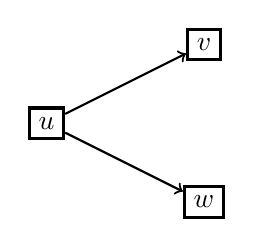
\begin{tikzpicture}[every node/.style={circle, draw, scale=1}, scale=1.0, rotate = 180]

\tikzset{every node/.style={draw, scale=1, very thick}} 
\node (today) at (3.0, 3.0) {$u$};
\node (tom1) at (1.0, 2.0) {$v$};
\node (tom2) at (1.0, 4.0) {$w$};

\tikzset{every node/.style={}}; 
\tikzset{mystyle/.style={->,thick}};  
\path (today) edge [mystyle] node {} (tom1);
\path (today) edge [mystyle] node {} (tom2);
\end{tikzpicture}
\end{center}
\caption{A frame}
\end{minipage}
\begin{minipage}[b]{0.4\linewidth}
\begin{center}
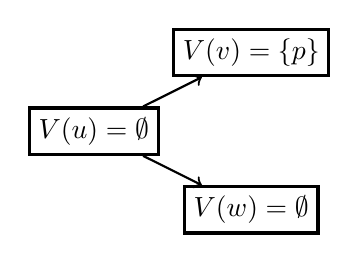
\begin{tikzpicture}[every node/.style={circle, draw, scale=1}, scale=1.0, rotate = 180]

\tikzset{every node/.style={draw, scale=1, very thick}} 
\node (today) at (3.0, 3.0) {$V(u) = \emptyset$};
\node (tom1) at (1.0, 2.0) {$V(v) = \{p\}$};
\node (tom2) at (1.0, 4.0) {$V(w) = \emptyset$};

\tikzset{every node/.style={}}; 
\tikzset{mystyle/.style={->,thick}};  
\path (today) edge [mystyle] node {} (tom1);
\path (today) edge [mystyle] node {} (tom2);
\end{tikzpicture}
\end{center}
\caption{A model}
\end{minipage}


\end{figure}

The mysterious ingredient is our \textit{Axiom K}: $\square(p \to q) \to \square p \to \square q$, or $(\square(p \to q) \wedge \square p) \to \square q$. (\textit{``If $p$ is necessarily true, and $p$ entails $q$ by necessity, then necessarily $q$ must also be true.''})

Together with (the soundness of) the Necessitation-rule (and uniform substitution), the $K$ axiom form some ``smallest'' assumptions about the behaviour of the modal connective; the \textit{normal modal logics}.

Our claim only relied on ``normality'' (very basic assumptions). What about the modality ``It is \textit{known} that $\ldots$''? If we use the box to model this modality, the necessitation-rule is the claim that ``All tautologies are known''. Philosophers often also insist that knowledge is \textit{veridical}. We can express this as the axiom $\square p \to p$ (we call this the Truth axiom, or just $T$). Other axioms stipulated in (a na\"ive) epistemic logic are: introspection; $\square p \to \square\square p$ and negative introspection $\neg \square p\to \square \neg \square p$, usually written $\lozenge p \to \square \lozenge p$ (\textit{Frame-equivalent}).
\subsection{Syntax}
$$\phi\quad ::= \quad p ~|~ \neg \phi ~|~ \phi \vee \phi ~|~ \lozenge \phi \quad\quad\text{( + abbreviations)}$$
\subsection{Semantics}
A SL-formula is evaluated against a ``truth table''. If $\prop$ is the set of propositional symbols, a configuration/instantiation/row in a truth table is some subset of $\prop$, and all possible configurations/instatiations/the entire truth table is the powerset $\wp(\prop)$.

We are not interested in ``which row is the right one'', we're interested in the \textit{validities}. Now, suppose we want to model the fact that it is not raining now, but it might (or might not) rain tomorrow. A \textit{state} is a day. 

\begin{figure}[ht]
\centering
\begin{tabular}{l|l}
\multicolumn{1}{c}{$\phi_F$ is} & \multicolumn{1}{|c}{$\phi_M$ is} \\ \hline
% & \textit{valid on the class of frames} $\mathsf F$ iff for all $\mathcal F \in \mathsf F$, $\mathcal F \Vdash \phi_M$ \\
\textit{valid} iff for all $M~:~M \vDash \phi_F$ & \textit{valid on a frame} $\mathcal F$ iff for all  $w \in \mathcal F$, $\mathcal F,w \Vdash \phi_M$\\
\textit{satisfied} in $M$ iff for all $v~:~M \vDash_v \phi_F$ & \textit{valid in a model } $M$ iff for every state $w$, $M, w \Vdash \phi_M$\\
\textit{true} w.r.t. $M$ and $v$ iff for $[\![\phi_F]\!]^M_v = 1$ & \textit{true}\footnote{Not very usual notation. Wrote it for comparison.} in $M$ at $w$ iff $w \in [\![\phi_M]\!]^M$\\
\end{tabular}
\end{figure}

Satisfaction of a formula $\phi$ in model $M = (W, R, V)$ at state $w$ is defined inductively: 
\begin{center}
\begin{tabular} {llcll}
$M, w \Vdash p $&$\iff~ p \in V(w)$ & \phantom{space} & $M, w \Vdash \phi \wedge \psi $&$\iff~ M, w \Vdash \phi \text{ and } M, w \Vdash \psi$ \\
$M, w \Vdash \neg \phi $&$\iff~ M, w \nVdash \phi$ & & $M, w \Vdash \lozenge \phi $&$\iff~ \textit{there is a }w'\in W \text{ s.t. } wRw' \text{ and } M, w' \Vdash \phi$\\
\end{tabular}
\end{center}

A Kripke model is a graph where each node is a ``SL model''. $M = (W, R, V)$ where $\bullet$ $W$ is a non-empty set of states, $\bullet R \subseteq W^2$ and $\bullet V : W \to 2^{\mathcal P}$ (coloring). A \textit{frame} is just the graph. We're usually not interested in \textit{all} graphs, but only those that satisfy certain conditions/axioms. 

\begin{proposition}Every frame satisfies the \textit{K} axiom ($\mathcal F \Vdash K$.)
\end{proposition}

\begin{proof} Let $\mathcal F$ be an arbitrary frame. Let $w$ be an arbitrary point in $\mathcal F$. Let $V$ be an arbitrary valuation over $\mathcal F$ such that $\mathcal F, V, w \Vdash \square(p \to q)$ and $\ff, V, w \Vdash \square p$ (otherwise we're done). Suppose $w$ has a neighbour $w'$ (otherwise we're done). Every $w'$ s.t. $wRw'$ satisfies $p \to q$ and $p$. It follows by MP that also every neighbour $w'$ satisfies $q$. Hence $\ff, V, w \Vdash \square q$.
\end{proof}

Certain logical axioms characterize classes of frames with certain properties. For example, the class of frames which satisfies the $T$ axiom are exactly the reflexive frames.

\begin{proposition} $\ff \Vdash T \iff Refl(\ff)$ ($T =\square p \to p \equiv^{\mathcal F} p \to \lozenge p$). \textcolor{magenta}{(Not for models; e.g., $\{p\} \to \{p\}\circlearrowleft$)}
\end{proposition}

\begin{proof} Two directions:  
\begin{description}
\item[$\Rightarrow$)] Suppose $\ff \Vdash \square p \to p$. Let $w$ be an arbitrary point and $V$ be a valuation over $\ff$ s.t. $V(w') = \{p\} \iff wRw'$. Clearly $\ff,V,w \Vdash \square p$. Since $\ff \Vdash \square p \to p$ we have, in particular $\ff, V, w\Vdash \square p \to p$ and hence, by MP, $\ff, V, w \vDash p$. By def. of $V$ we get $wRw$.
\item[$\Leftarrow)$] Notice: $\square p \to p$ and $p \to \lozenge p$ are \textit{frame equivalent}. Suppose $\ff$ is reflexive. Let $w$ be an arbitrary point in $\ff$. Let $V$ any valuation. (If $\ff, V, w \nVdash p$, we're done.) Suppose $\ff, V, w \Vdash p$, then there is a neighbour, $w$ itself, which satisfies $p$, hence $\ff, V, w \Vdash \lozenge p$.
\end{description}
\end{proof}

Similar proofs gives us $4: \square p \to \square\square p \sim$transitive, $5:\lozenge p \to \square \lozenge p\sim$Euclidean, $B: p \to \square \lozenge p \sim$symmetric, etc...

\subsection{Equivalence/Similarity}
Equivalence is defined straightforwardly:
\begin{definition}Let $\mm, \mm'$ be models and $w,w'$ be states in them.
\begin{align*}
(\mm,w) \leftrightsquigarrow (\mm',w') &\iff \{\phi ~|~ \mm, w \Vdash \phi\} = \{\phi ~|~ \mm', w' \Vdash \phi\} \\
\mm \leftrightsquigarrow \mm' &\iff \{\phi ~|~ \mm \Vdash \phi\} = \{\phi ~|~ \mm' \Vdash \phi\}\\
\end{align*}
\end{definition}

\begin{proposition} Satisfaction is invariant under generated submodels. 
\end{proposition}

\begin{proof}Let $\mm'$ be a generated submodel of $\mm$ ($\mm' \rightarrowtail \mm$), i.e., $\mm' = (W', R', V') \subseteq \mm = (W, R, V)$ s.t. 
$$V' = V|_{W'}\text{, }R' = R\cap W'^2 \text{ and for all } w \in W' ~:~ wRw'\Rightarrow  w'\in W'$$
Need to show that $w \in W'$, $\mm, w \Vdash \phi \iff \mm', w \Vdash \phi$. Structural induction on $\phi$: 
\begin{description}
\item[Base case ($p$)] Trivial.
\item[Induction step (show only $\lozenge \phi$)] Suppose $\mm, w \Vdash \lozenge \phi$. Let $w'$ be the state s.t. $wRw'$ and $\mm,w' \Vdash \phi$. By the IH we have $\mm',w'\Vdash \phi$. Since $w,w' \in W'$, $R' = R\cap W'^2$, and $(w,w') \in R$ we have $(w,w') \in R'$ and hence $\mm', w\Vdash \lozenge\phi$.\\
Suppose $\mm', w\Vdash \lozenge\phi$, then there is a state $w'$ s.t. $(w,w') \in R'$ ($\subseteq R \Rightarrow (w,w') \in R$) and $\mm', w' \Vdash \phi$. By IH we have $\mm, w'\Vdash \phi$ and the claim follows.
\end{description}
\end{proof}

Equivalence is not as fine-grained as we would like, however. 

\begin{figure}[ht]
\centering
\begin{minipage}[b]{0.35\linewidth}
\begin{center}
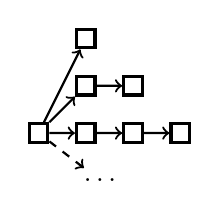
\begin{tikzpicture}[every node/.style={circle, draw, scale=1}, scale=0.6, rotate = 180]

\tikzset{every node/.style={draw, scale=1, very thick}} 
\node (11) at (3.0, 5.0) {};
\node (12) at (2.0, 3.0) {};
\node (21) at (2.0, 4.0) {};
\node (22) at (1.0, 4.0) {};
\node (31) at (2.0, 5.0) {};
\node (32) at (1.0, 5.0) {};
\node (33) at (0.0, 5.0) {};
\tikzset{every node/.style={scale=1, very thick}} 
\node (ddd) at (1.7, 6.0) {$\dots$};

\tikzset{every node/.style={}}; 
\tikzset{mystyle/.style={->,thick}};  
\path (11) edge [mystyle] node {} (12);
\path (11) edge [mystyle] node {} (21);
\path (21) edge [mystyle] node {} (22);
\path (11) edge [mystyle] node {} (31);
\path (31) edge [mystyle] node {} (32);
\path (32) edge [mystyle] node {} (33);
\tikzset{mystyle/.style={->,thick,dashed}};  
\path (11) edge [mystyle] node {} (ddd);
\end{tikzpicture}
\end{center}
\end{minipage}
\begin{minipage}[b]{0.35\linewidth}
\begin{center}
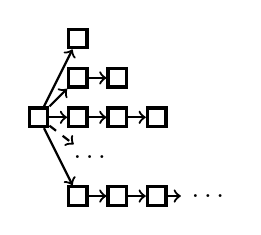
\begin{tikzpicture}[every node/.style={circle, draw, scale=1}, scale=0.5, rotate = 180]

\tikzset{every node/.style={draw, scale=1, very thick}} 
\node (11) at (3.0, 5.0) {};
\node (12) at (2.0, 3.0) {};
\node (21) at (2.0, 4.0) {};
\node (22) at (1.0, 4.0) {};
\node (31) at (2.0, 5.0) {};
\node (32) at (1.0, 5.0) {};
\node (33) at (0.0, 5.0) {};
\node (inf1) at (2.0, 7.0) {};
\node (inf2) at (1.0, 7.0) {};
\node (inf3) at (0.0, 7.0) {};
\tikzset{every node/.style={scale=1, very thick}} 
\node (infddd) at (-1.3, 7.0) {$\dots$};
\node (ddd) at (1.7, 6.0) {$\dots$};

\tikzset{every node/.style={}}; 
\tikzset{mystyle/.style={->,thick}};  
\path (11) edge [mystyle] node {} (12);
\path (11) edge [mystyle] node {} (21);
\path (21) edge [mystyle] node {} (22);
\path (11) edge [mystyle] node {} (31);
\path (31) edge [mystyle] node {} (32);
\path (32) edge [mystyle] node {} (33);
\path (11) edge [mystyle] node {} (inf1);
\path (inf1) edge [mystyle] node {} (inf2);
\path (inf2) edge [mystyle] node {} (inf3);
\path (inf3) edge [mystyle] node {} (infddd);

\tikzset{mystyle/.style={->,thick,dashed}};  
\path (11) edge [mystyle] node {} (ddd);
\end{tikzpicture}
\end{center}
\end{minipage}
\caption{Equivalent, but not bisimilar}
\end{figure}

We have natural notions of relations between (Kripke) structures. 
\begin{definition}\textbf{(Homomorphisms)} Let $M = (W, R, V), M' = (W', R', V')$ be models. A \textit{homomorphism}, denoted $f:M \to M'$, is a map $f:W \to W'$ s.t.
\begin{itemize}
\item for each $p$ and each $w \in W$, if $w \in V(p)$ then $f(w) \in V'(p)$ [[or $V(w) \subseteq V'(f(w))$]]
\item if $wRv$, then $f(w)R'f(v)$.
\end{itemize}
(A homomorphism $f : \ff \to \ff'$ for \textit{frames} from $\ff = (W, R)$ to $\ff' = (W',R')$ is a map $f:W \to W'$ s.t. $wRv~\Rightarrow~f(w)R'f(v)$.)
\end{definition}

Homomorphisms are a natural notion for relations between structures, but it doesn't yield any invariance w.r.t. satisfaction of (modal) logical formulas. \textcolor{magenta}{(A neighbourless point satisfies $\square \bot$, there is a homomorphism into a reflexive point which doesn't.)}

We could strengthen the requirement:
\begin{definition}\textbf{(Strong homomorphism)} As above, but:
\begin{itemize}
\item $w \in V(p) \iff f(w) \in V'(p)$ [[or $V(w) = V'(f(w))$]]
\item $wRv$ \textit{iff} $f(w)R'f(v)$
\end{itemize}
\end{definition}

This gives some invariance results (e.g., $\bullet$ surjective strong homom. $f : M \to M'$, then $w \meq f(w)$, $\bullet$ $M \iso M' \Rightarrow M \meq M'$.), 
but many morphisms which give invariance fail to be strong homomorphisms \textcolor{magenta}{(e.g., $f : \{u \to v \circlearrowleft\} \to \{w\circlearrowleft\}$)}. Isomorphisms are bijective strong homomorphisms.

\begin{definition}\textbf{(Bounded Morphisms)} Let $f: M = (W, R, V) \to M' = (W', R', V')$ be a homomorphism s.t.
\begin{itemize}
\item $p \in V(w)$ \textit{iff} $p \in V'(f(w))$
\item \textit{moot bc homom.:} $wRv$ then $f(w)Rf(v)$, and
\item $f(w)R'v' \Rightarrow$ $wRv$ for some $v$ s.t. $f(v) = v'$ (the \textit{Back} condition).
\end{itemize}
\end{definition}

\begin{figure}[ht]
\begin{minipage}[b]{0.4\linewidth}
\begin{center}
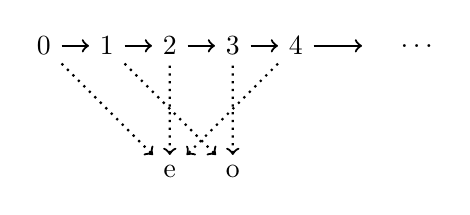
\begin{tikzpicture}[every node/.style={circle, draw, scale=1}, scale=0.8, rotate = 180]
\tikzset{every node/.style={scale=1, very thick}} 
\node (n0) at (5.0, 0.0) {0};
\node (n1) at (4.0, 0.0) {1};
\node (n2) at (3.0, 0.0) {2};
\node (n3) at (2.0, 0.0) {3};
\node (n4) at (1.0, 0.0) {4};
\node (ddd) at (-0.7, 0.0) {$\quad\dots$};
\node (e) at (3.0, 2.0) {e};
\node (o) at (2.0, 2.0) {o};

\tikzset{every node/.style={}}; 
\tikzset{mystyle/.style={->,thick}};  
\path (n0) edge [mystyle] node {} (n1);
\path (n1) edge [mystyle] node {} (n2);
\path (n2) edge [mystyle] node {} (n3);
\path (n3) edge [mystyle] node {} (n4);
\path (n4) edge [mystyle] node {} (ddd);

\tikzset{mystyle/.style={->,thick,dotted}};  
\path (n0) edge [mystyle] node {} (e);
\path (n1) edge [mystyle] node {} (o);
\path (n2) edge [mystyle] node {} (e);
\path (n3) edge [mystyle] node {} (o);
\path (n4) edge [mystyle] node {} (e);
\end{tikzpicture}
\end{center}
\caption{Bounded, not strong (one way!)}
\end{minipage}
\begin{minipage}[b]{0.4\linewidth}
\begin{center}
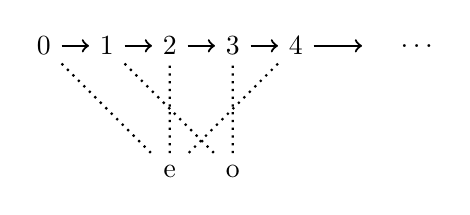
\begin{tikzpicture}[every node/.style={circle, draw, scale=1}, scale=0.8, rotate = 180]
\tikzset{every node/.style={scale=1, very thick}} 
\node (n0) at (5.0, 0.0) {0};
\node (n1) at (4.0, 0.0) {1};
\node (n2) at (3.0, 0.0) {2};
\node (n3) at (2.0, 0.0) {3};
\node (n4) at (1.0, 0.0) {4};
\node (ddd) at (-0.7, 0.0) {$\quad\dots$};
\node (e) at (3.0, 2.0) {e};
\node (o) at (2.0, 2.0) {o};

\tikzset{every node/.style={}}; 
\tikzset{mystyle/.style={->,thick}};  
\path (n0) edge [mystyle] node {} (n1);
\path (n1) edge [mystyle] node {} (n2);
\path (n2) edge [mystyle] node {} (n3);
\path (n3) edge [mystyle] node {} (n4);
\path (n4) edge [mystyle] node {} (ddd);

\tikzset{mystyle/.style={-,thick,dotted}};  
\path (n0) edge [mystyle] node {} (e);
\path (n1) edge [mystyle] node {} (o);
\path (n2) edge [mystyle] node {} (e);
\path (n3) edge [mystyle] node {} (o);
\path (n4) edge [mystyle] node {} (e);
\end{tikzpicture}
\end{center}
\caption{Bisimilar (coming up)}
\end{minipage}
\end{figure}


\subsection{Bisimulation}
\begin{definition} If $M = (W, R, V)$ and $M' = (W', R', V')$ are models and $Z \subseteq W \times W'$, then $M \bisim M'$ \textit{iff}
\begin{description}
\item[Propositional agreement] if $wZw'$, then $V(w) = V'(w')$, 
\item[Forth] If $wZw'$ and $wRv$, then there is a $v'$ s.t. $vZv'$ and $w'R'v'$, and
\item[Back] If $wZw'$ and $w'R'v'$, then there is a $v$ s.t. $vZv'$ and $wRv$.
\end{description}
\end{definition}

\begin{figure}[ht]
\begin{minipage}[b]{0.3\linewidth}
\begin{center}
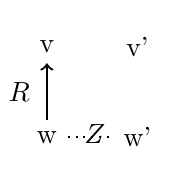
\begin{tikzpicture}[every node/.style={circle, draw, scale=1}, scale=0.23, rotate = 180]
\tikzset{every node/.style={scale=1, very thick}} 
\node (w) at (5.0, 5.0) {w};
\node (v) at (5.0, 0.0) {v};
\node (ww) at (0.0, 5.0) {w'};
\node (vv) at (0.0, 0.0) {v'};
\tikzset{every node/.style={scale=1, very thick}} 

\tikzset{every node/.style={}}; 
\tikzset{mystyle/.style={->,thick}};  
\path (w) edge [mystyle] node {$\hspace{-2em}R$} (v);
\tikzset{mystyle/.style={-,thick,dotted}};  
\path (w) edge [mystyle] node {$\begin{matrix} \\ Z \end{matrix}$} (ww);

\tikzset{mystyle/.style={->,thick,dashed}};  
\end{tikzpicture}
\end{center}
\end{minipage}
\begin{minipage}[b]{0.3\linewidth}
\begin{center}
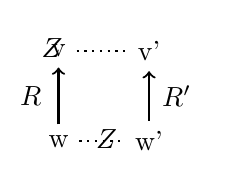
\begin{tikzpicture}[every node/.style={circle, draw, scale=1}, scale=0.23, rotate = 180]
\tikzset{every node/.style={scale=1, very thick}} 
\node (w) at (5.0, 5.0) {w};
\node (v) at (5.0, 0.0) {v};
\node (ww) at (0.0, 5.0) {w'};
\node (vv) at (0.0, 0.0) {v'};
\tikzset{every node/.style={scale=1, very thick}} 

\tikzset{every node/.style={}}; 
\tikzset{mystyle/.style={->,thick}};  
\path (w) edge [mystyle] node {$\hspace{-2em}R$} (v);
\path (ww) edge [mystyle] node {$\hspace{2em}R'$} (vv);
\tikzset{mystyle/.style={-,thick,dotted}};  
\path (w) edge [mystyle] node {$\begin{matrix} \\ Z \end{matrix}$} (ww);
\path (v) edge [mystyle] node {$\begin{matrix} Z \\ \phantom{Haxord!}\end{matrix}$} (vv);

\tikzset{mystyle/.style={->,thick,dashed}};  
\end{tikzpicture}
\end{center}
\end{minipage}
\begin{minipage}[b]{0.3\linewidth}
\begin{center}
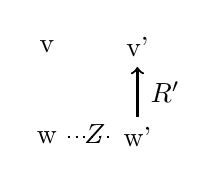
\begin{tikzpicture}[every node/.style={circle, draw, scale=1}, scale=0.23, rotate = 180]
\tikzset{every node/.style={scale=1, very thick}} 
\node (w) at (5.0, 5.0) {w};
\node (v) at (5.0, 0.0) {v};
\node (ww) at (0.0, 5.0) {w'};
\node (vv) at (0.0, 0.0) {v'};
\tikzset{every node/.style={scale=1, very thick}} 

\tikzset{every node/.style={}}; 
\tikzset{mystyle/.style={->,thick}};  
\path (ww) edge [mystyle] node {$\hspace{2em}R'$} (vv);
\tikzset{mystyle/.style={-,thick,dotted}};  
\path (w) edge [mystyle] node {$\begin{matrix} \\ Z \end{matrix}$} (ww);

\tikzset{mystyle/.style={->,thick,dashed}};  
\end{tikzpicture}
\end{center}
\end{minipage}
%\caption*{Forth $\Longrightarrow\hspace{14em}\Longleftarrow$ Back}
\end{figure}

\begin{proposition}Modal formulas are invariant under bisimulation ($w \bisim w' \Rightarrow w \leftrightsquigarrow w'$).
\label{prop:bisim-imp-eq}
\end{proposition}

\begin{proof}Let $M,w$ and $M',w'$ be pointed models such that $w \bisim w'$. Induction on $\phi$. 
\begin{description}
\item[Base case ($p$)] By def.
\item[Induction step: ($\lozenge \phi$)] Suppose $M, w \Vdash \lozenge \phi$, then $wRv$ and $M, v \Vdash \phi$. But since $w\bisim w'$, there is a $v'$ s.t. $w'R'v'$ and $v \bisim v'$. By IH it follows that $M', v' \Vdash \phi$, and hence $M', w \Vdash \lozenge\phi$.
\end{description}
\end{proof}
When is the converse true? 
\begin{proposition} (\textbf{Hennessy-Milner Theorem}) Let $M = (W, R, V)$ and $M' = (W', R', V')$ be two \textit{image-finite} models (every $w$, $|R_{trg}(w)| \in \mathbb N$). For every $w \in W$ and $w' \in W'$, $w \bisim w' \iff w \leftrightsquigarrow w'$. 
\end{proposition}

\begin{proof}
$\Rightarrow$) is done (Prop. \ref{prop:bisim-imp-eq}). $\Leftarrow$) Prove that $\leftrightsquigarrow$ is a bisimulation relation on these models.

$\leftrightsquigarrow$ clearly satisfies \textbf{Propositional Agreement}. Now, for \textbf{Forth}, suppose $w \leftrightsquigarrow w'$ and $wRv$. Suppose towards a contradiction that there is no $v'$ in $M'$ such that $w'R'v'$ and $v \meq v'$. Notice:
\begin{itemize}
\item $M, w \Vdash \lozenge \top$ (has a successor), and since $w \meq w'$, 
\item $R_{trg}(w')$ is non-empty and finite (from \textit{image-finite}).
\end{itemize}
Let's say $R_{trg}(w') = \{w_1', w_2', \dots, w_n'\}$. By assumption (no $v' \in R_{trg}(w') \meq v \in R_{trg}(w)$), there is a formula for each $w_i'$, say $\psi_i$ s.t. $M, v \Vdash \psi_i$, but $M', w_i' \Vdash \psi_i$ (otherwise they would be equivalent!). But then 
$$M, w \Vdash \lozenge (\psi_1 \wedge \dots \wedge \psi_n) \text{ and } M', w' \nVdash \lozenge(\psi_1 \wedge \ldots \wedge \psi_n)$$
which contradicts our assumption that $w \meq w'$. \textcolor{magenta}{Using the fact that formulas are finite.}
\end{proof}

Bisimulation is cool because:\begin{enumerate}
\item It's behavioural/observational like we want when talking about LTSs.
\item It's is a more fine-grained measure of similarity than equivalence, but not so fine-grained that it distinguishes modally indistinguishable models.
\item ``The quotient of a model w.r.t. its largest auto-bisimulation can be regarded as a minimal representation of this model.'' [BB]
\item Two non-wellfounded sets are considered equal if their decoration graphs are bisimilar. [$\sim$BB]
\item Modal logic is \textit{the} fragment of FOL which is closed under bisimulation (van Benthem Characterization Theorem).
\end{enumerate}

\subsection{Frames as coalgebras}
A frame is a graph $(W, R)$. The relation $R$ can be represented as a map $W \to \wp(W)$, i.e., a morphism in $\mathsf{Set}$. And waddayano, it fits our coalg(functor)-picture. 

\begin{figure}[ht]
\begin{minipage}[b]{0.5\linewidth}
\begin{center}
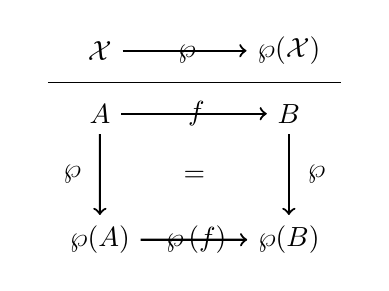
\begin{tikzpicture}[every node/.style={circle, draw, scale=1}, scale=0.8, rotate = 180]

\tikzset{every node/.style={scale=1, very thick}} 
\node (x) at (3.0, 0.0) {$\xx$};
\node (sx) at (0.0, 0.0) {$\wp(\xx)$};

\node (e0) at (4.0, 0.5) {};
\node (e1) at (-1.0, 0.5) {};
\node (eq) at (1.5, 2.0) {$=$};

\node (A) at (3.0, 1.0) {$A$};
\node (B) at (0.0, 1.0) {$B$};
\node (pA) at (3.0, 3.0) {$\wp(A)$};
\node (pB) at (0.0, 3.0) {$\wp(B)$};

\tikzset{every node/.style={}}; 
\tikzset{mystyle/.style={-,thin}};  
\path (e0) edge [mystyle] node {} (e1);
\tikzset{mystyle/.style={->,thick}};  
\path (x) edge [mystyle] node {$\begin{matrix} \wp \\ \\ \end{matrix}$} (sx);

\tikzset{mystyle/.style={->,thick}};  
\path (A) edge [mystyle] node {$\begin{matrix} f \\ \\ \end{matrix}$} (B);
\path (pA) edge [mystyle] node {$\begin{matrix} \wp(f) \\ \\ \end{matrix}$} (pB);
\path (A) edge [mystyle] node {$\wp\hspace{2em}$} (pA);
\path (B) edge [mystyle] node {$\hspace{2em}\wp$} (pB);

\end{tikzpicture}
\end{center}
\caption{$\wp$ is an endo-functor on $\mathsf{Set}$}
\label{fig:frame-in-set}
\end{minipage}
\begin{minipage}[b]{0.45\linewidth}
\begin{center}
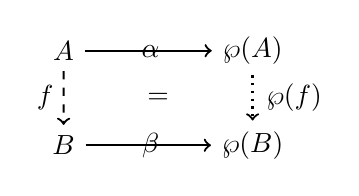
\begin{tikzpicture}[every node/.style={circle, draw, scale=1}, scale=0.8, rotate = 180]
\tikzset{every node/.style={scale=1, very thick}} 
\node (A) at (3.0, 0.0) {$A$};
\node (sA) at (0.0, 0.0) {$\wp(A)$};
\node (B) at (3.0, 1.5) {$B$};
\node (sB) at (0.0, 1.5) {$\wp(B)$};

\node (commute) at (1.5, 0.75) {$=$};

\tikzset{every node/.style={}}; 
\tikzset{mystyle/.style={->,thick}};  
\path (A) edge [mystyle] node {$\begin{matrix} \alpha \\ \\ \end{matrix}$} (sA);
\path (B) edge [mystyle] node {$\begin{matrix} \beta \\ \\ \end{matrix}$} (sB);
\tikzset{mystyle/.style={->,thick,dashed}};  
\path (A) edge [mystyle] node {$f~\quad$} (B);
\tikzset{mystyle/.style={->,thick,dotted}};  
\path (sA) edge [mystyle] node {$\hspace{3em} \wp(f)$} (sB);

\end{tikzpicture}
\end{center}
\caption{Frames as $(A,\alpha)$ (coalg) in $\mathsf{Set}$}
\label{fig:morphism-in-frame}
\end{minipage}
\end{figure}

\begin{figure}[ht]
\begin{center}
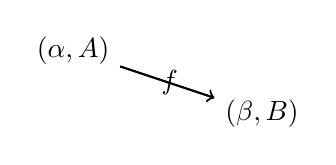
\begin{tikzpicture}[every node/.style={circle, draw, scale=1}, scale=0.8, rotate = 180]

\tikzset{every node/.style={scale=1, very thick}} 
\node (x) at (3.0, 0.0) {$(\alpha,A)$};
\node (sx) at (0.0, 1.0) {$(\beta, B)$};

\tikzset{every node/.style={}}; 
\tikzset{mystyle/.style={->,thick}};  
\path (x) edge [mystyle] node {$\begin{matrix} f \\ \\ \end{matrix}$} (sx);
\end{tikzpicture}
\end{center}
\caption{Frames as obj in $\mathsf{Coalg}(\wp)$}
\label{fig:frame-coalg}
\end{figure}

A functor is a map $F : \mathbb C \to \mathbb D$ such that $\bullet$ for any object $c$ in $\mathbb C$, $F(c)$ is an object in $\mathbb D$, $\bullet$ when $f : c \to c'$ is a morphism in $\mathbb C$, then $F(f) : F(c) \to F(c')$ is a morphism in $\mathbb D$, $\bullet~$ $F(Id_c) = Id_{F(c)}$, and $\bullet ~ F(f;g) = F(f);F(g)$.

\begin{proposition}\textbf{Figure \ref{fig:frame-in-set}} is an (endo-)functor in $\mathsf{Set}$ .\end{proposition}

\begin{proof} Let $f : A \to B$. $\wp(f)(S) = \{f(x) ~|~ x \in S\}$. 

$F(f;g)(S) = \{ (f;g)(x) ~|~ x \in S\} = \{ g(y) ~|~ y = f(x), x \in S\} =  \{g (y) ~|~ y \in \{ f(x) ~|~ x \in S\}\} = \{g (y) ~|~ y \in F(f)(S)\} $\\
$= (F(f);F(g))(S)$
\end{proof}

\textbf{Figure \ref{fig:morphism-in-frame}} is just like half of Figure \ref{fig:frame-in-set}, but nicer, rotated, and a bit squashed.

\begin{definition}
Morphisms in $\mathsf{Coalg}(\wp)$ ($f : (\alpha, A) \to (\beta, B)$ in \textbf{Figure \ref{fig:frame-coalg}}) are maps $f : A \to B$ such that 
\begin{enumerate}
\item $y \in \alpha(x) ~\Rightarrow~ f(y) \in \beta(f(x))$ [[or $x(\alpha)y ~\Rightarrow~ f(x)(\beta)f(y)$, or $xRy ~\Rightarrow~ f(x)R'f(y)$]]
\item $y' \in \beta(f(x)) \Rightarrow \exists y$ s.t. $y \in \alpha(x)$ and $f(y) = y'$.
\end{enumerate}
\end{definition}
\begin{figure}[ht]
\centering
\begin{minipage}[b]{0.5\linewidth}
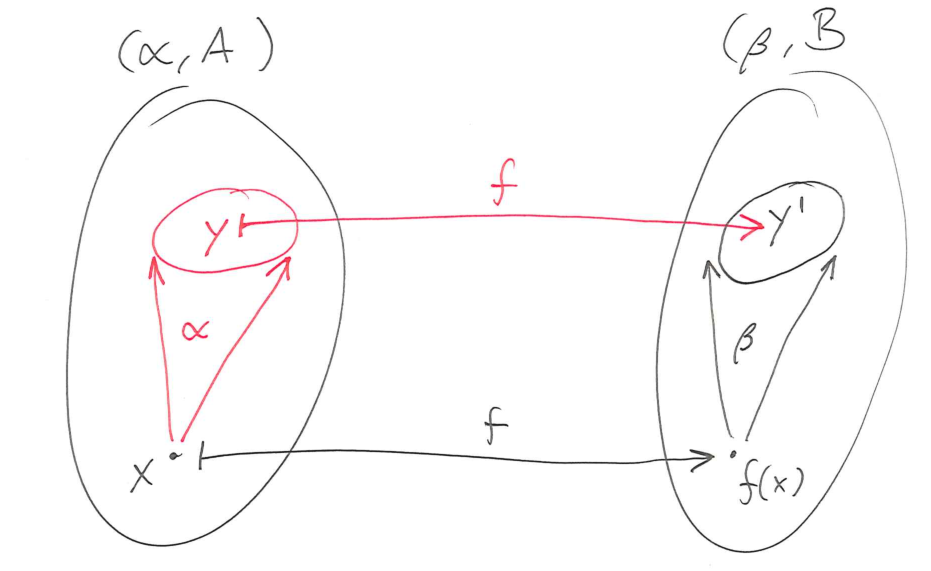
\includegraphics[scale=0.4]{frame-coalg-morphism-2.pdf}
\end{minipage}
\begin{minipage}[b]{0.4\linewidth}
That is to say:
\begin{enumerate}
\item $f_{\wp}(\alpha(x)) \subseteq \beta(f(x))$, and
\item $\beta(f(x)) \subseteq f_\wp(\alpha(x))$
\end{enumerate}

Or just 
$$\alpha;f_\wp = f;\beta$$
$\vspace{3em}$
\end{minipage}
\caption{(2) says ``If $f:(\alpha, A) \to (\beta, B)$ and we've got the black, we also have the red''.}
\end{figure}



\subsection{Models as coalgebras}
Models have type-functor $F : \xx \to \wp(\prop) \times \wp(\xx)$. Since we don't care about all the propositional symbols we can simplify to $F : \xx \to C \times \wp(\xx)$. We can think of an element in $C$ as a row in a truthtable or a color or whatever.

\begin{figure}[ht]
\centering
\begin{minipage}[b]{0.4\linewidth}
\begin{center}
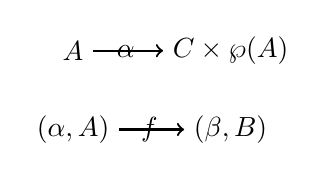
\begin{tikzpicture}
\node (A) at (0.0, 1.0) {$A$};
\node (trg) at (2.0, 1.0) {$C\times\wp(A)$};
\node (aA) at (0.0, 0.0) {$(\alpha, A)$};
\node (bB) at (2.0, 0.0) {$(\beta, B)$};

\tikzset{mystyle/.style={->,thick}};  
\path (A) edge [mystyle] node {$\begin{matrix}\alpha \\~ \end{matrix}$} (trg);
\path (aA) edge [mystyle] node {$\begin{matrix}f \\ ~\end{matrix}$} (bB);
\end{tikzpicture}
\end{center}
\caption{Model \& Morphism}
\label{fig:coalg-mod-and-morph}
\end{minipage}
\begin{minipage}[b]{0.5\linewidth}
\begin{center}
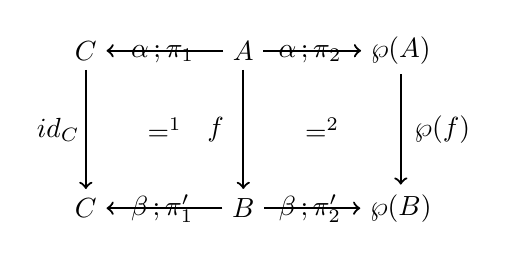
\begin{tikzpicture}
\node (A) at (0.0, 2.0) {$A$};
\node (B) at (0.0, 0.0) {$B$};

\node (CA) at (-2.0, 2.0) {$C$};
\node (sA) at (2.0, 2.0) {$\wp(A)$};

\node (CB) at (-2.0, 0.0) {$C$};
\node (sB) at (2.0, 0.0) {$\wp(B)$};

\node (eq2) at (-1.0, 1.0) {$=^1$};
\node (eq1) at (1.0, 1.0) {$=^2$};

\tikzset{mystyle/.style={->,thick}};  
\path (A) edge [mystyle] node {$f\hspace{2em}$} (B);
\path (A) edge [mystyle] node {$\begin{matrix}\alpha;\pi_1 \\ ~\end{matrix}$} (CA);
\path (A) edge [mystyle] node {$\begin{matrix}\alpha;\pi_2 \\ ~\end{matrix}$} (sA);

\path (B) edge [mystyle] node {$\begin{matrix}\beta;\pi'_1 \\ ~\end{matrix}$} (CB);
\path (B) edge [mystyle] node {$\begin{matrix}\beta;\pi'_2 \\ ~\end{matrix}$} (sB);

\path (CA) edge [mystyle] node {$id_C\hspace{2em}$} (CB);
\path (sA) edge [mystyle] node {$\hspace{3em}\wp(f)$} (sB);
\end{tikzpicture}
\end{center}
\caption{Morphism condition}
\label{fig:mod-morph-cond}
\end{minipage}
\end{figure}

\begin{figure}[ht]
\begin{center}
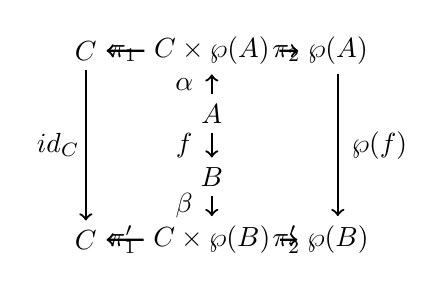
\begin{tikzpicture}[scale=0.4]
\node (A) at (0.0, 2.0) {$A$};
\node (CxpA) at (0.0, 4.0) {$C\times\wp(A)$};
\node (B) at (0.0, 0.0) {$B$};
\node (CxpB) at (0.0, -2.0) {$C \times \wp(B)$};

\node (CA) at (-4.0, 4.0) {$C$};
\node (sA) at (4.0, 4.0) {$\wp(A)$};

\node (CB) at (-4.0, -2.0) {$C$};
\node (sB) at (4.0, -2.0) {$\wp(B)$};

\tikzset{mystyle/.style={->,thick}};  
\path (A) edge [mystyle] node {$f\hspace{2em}$} (B);

\path (A) edge [mystyle] node {$\alpha\hspace{2em}$} (CxpA);
\path (B) edge [mystyle] node {$\beta\hspace{2em}$} (CxpB);

\path (CA) edge [mystyle] node {$id_C\hspace{2em}$} (CB);
\path (sA) edge [mystyle] node {$\hspace{3em}\wp(f)$} (sB);

\path (CxpA) edge [mystyle] node {$\begin{matrix}{\pi_1} \\ ~\end{matrix}$} (CA);
\path (CxpA) edge [mystyle] node {$\begin{matrix}{\pi_2} \\ ~\end{matrix}$} (sA);

\path (CxpB) edge [mystyle] node {$\begin{matrix}{\pi'_1} \\ ~\end{matrix}$} (CB);
\path (CxpB) edge [mystyle] node {$\begin{matrix}{\pi'_2} \\ ~\end{matrix}$} (sB);
\end{tikzpicture}
\end{center}
\caption{More verbose}
\end{figure}
\begin{minipage}[b]{0.6\linewidth}
A morphism in $\mathsf{Coalg}(C\times \wp)$ is a map $f : (\alpha, A) \to (\beta, B)$ (as in Figure \ref{fig:coalg-mod-and-morph}), such that the diagram in Figure \ref{fig:mod-morph-cond} commutes.

In Figure \ref{fig:mod-morph-cond} the two statements express ($=^1$): $a \in A$ and $f(a) \in B$ have the same coloring, and ($=^2$): the same as for frames (simulation).

Let's look at an example of two objects in $\mathsf{Coalg}(C\times \wp)$: 
\end{minipage}
\begin{minipage}[b]{0.3\linewidth}
\begin{center}
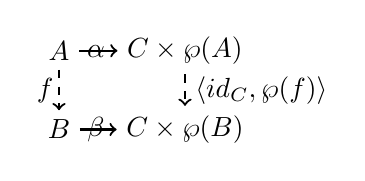
\begin{tikzpicture}
\node (A) at (0.0, 1.0) {$A$};
\node (trgA) at (1.6, 1.0) {$C\times\wp(A)$};
\node (B) at (0.0, 0.0) {$B$};
\node (trgB) at (1.6, 0.0) {$C\times\wp(B)$};

\tikzset{mystyle/.style={->,thick}};  
\path (A) edge [mystyle] node {$\begin{matrix}\alpha \\~ \end{matrix}$} (trgA);
\path (B) edge [mystyle] node {$\begin{matrix}\beta \\ ~\end{matrix}$} (trgB);
\tikzset{mystyle/.style={->,thick,dashed}};  
\path (A) edge [mystyle] node {$f\quad$} (B);
\path (trgA) edge [mystyle] node[right]{$\langle id_C, \wp(f) \rangle$} (trgB);
\end{tikzpicture}\\
\textsc{Actual Figure 13. } 
\end{center}
\end{minipage}


Let $A = \{1, 2, 3, 4, 5\}$, and $\alpha(1) = (c_1, \{2\}), \alpha(2) = (c_2, \{3\}), \alpha(3) = (c_1, \{4, 5\}) \alpha(4) = (c_2, \emptyset)$, and $\alpha(5) = (c_2, \emptyset)$.

Let $B = \{a, b, c, d, e\}$, and $\beta(a) = (c_1, \{b, c\}), \beta(b) = (c_2, \{d\}), \beta(c) = (c_2, \{d\}), \beta(d) = (c_1, \{e\})$, and $\beta(e) = (c_2, \emptyset)$.

Is there a morphism from $(\alpha, A)$ to $(\beta, B)$? Indeed there is. Let $f = \{1 \mapsto a, 2 \mapsto b, 3 \mapsto b, 4 \mapsto e, 5 \mapsto e\}$.



\subsection{Canonical models are final objects}
The elements in the category $\mathsf{Coalg}(\wp(P)\times\wp(A)) = \mathcal C$ are extactly all Kripke models (all models over arbitrary frames). Let $\mathfrak M^C$ be the canonical model for the the logic \textit{K}. A morphism in $\mathcal C$ is a bounded morphism from one model to another (as sketched above), i.e., a map from states to states such that (...)

\begin{proposition}
The unique bounded morphism $id_{\mathfrak M^C} : \mathfrak M^C \to \mathfrak M^C$ is the identity map (mapping each state (maximal consistent set of formulas) to itself).\end{proposition}


\begin{proof} Two claims:
\begin{description}
\item[Bounded morphism] the identity map $id_{\mathfrak M^C}$ is a bounded morphism.
\item[Unique] Suppose there was a bounded morphism $f : \mathfrak M^C \to \mathfrak M^C$ distinct from the identity map. Then there is some state $w$ such that $w \neq f(w)$. Let $\phi \in w$. We show that $\phi \in f(w)$. We prove the claim $\phi \in w \Leftrightarrow \phi \in f(w)$ by induction on $\phi$:
\begin{description}
\item[Base case ($p$)] $p \in w \Leftrightarrow w \Vdash p$, but since $f$ is a bounded morphism, $f(w) \Vdash p$, so $p \in f(w)$.
\item[Induction step(s)] Boolean cases are simple.
\begin{description}
\item[$\phi = \neg \psi$] $\neg \psi \in w \Leftrightarrow \psi \notin w$ (by the construction of $\mathfrak M^C$). By IH $\psi \notin f(w)$, and hence $\neg \psi \in f(w)$ (by construction).
\item[$\phi = \psi_1 \wedge \psi_2$] $\psi_1 \wedge \psi_2 \in w \Leftrightarrow \text{both } \psi_1 \in w \text{ and } \psi_2 \in w$ (corrolary from construction). IH yields $\psi_1,\psi_2 \in f(w)$ and definition of $\mathfrak M^C$ yields $\psi_1 \wedge \psi_2 \in f(w)$.
\item[$\phi = \lozenge \psi$] Let $v$ be an arbitrary state such that $wR^Cv$ and $v \Vdash \psi$. Since $f$ is a bounded morphism, $f(w)R^Cf(v)$. IH gives $f(v) \Vdash \psi$, but then $f(w)\Vdash \lozenge \psi$.
\end{description}
\end{description}
So $\phi \in w \Leftrightarrow \phi \in f(w)$ and $f$ needs to be the identity map.
\end{description}
So $id_{\mathfrak M^C}$ is the unique bounded morphism in $\mathcal C$ from $\mathfrak M^C$ to itself.
\end{proof}

A morphism from an arbitrary model into the canonical model is unique modulo the choice of how to extend a set of formulas to maximal sets.
\begin{proof} Here is a quote:
\begin{quote}
Grif: ``You can't call dibs on a spaceship! That's ridiculous!''
\begin{flushright}
from \textit{Red vs. Blue}, Season 5, Ep. \textit{``You can't park here''}
\end{flushright}
\end{quote}
\end{proof}

